% \documentclass[a4format,11pt]{article}
% \usepackage[utf8]{inputenc}
% \usepackage[T2A]{fontenc}
% \usepackage[english,russian]{babel}
% \usepackage{lipsum}
% \usepackage{amsmath}
% \usepackage[right=2cm,left=2cm,top=1cm,bottom=2cm]{geometry}
% \usepackage{graphicx}
% \usepackage{float}
% \usepackage{diagbox}
% \usepackage{multicol}

% \setcounter{secnumdepth}{0}

\author{А. Виленкин, Ю. Ионин}
\title{Площадь и интеграл}
\date{1977}


% \begin{document}
\maketitle
\begin{multicols}{2}
{\small\textbf{Из статьи В. Болтянского "О понятиях площади и объема", помещенной в этом номере, вы узнали
    об определении и различных способах вычисления площадей. Наиболее универсальным из них является применение интегрального исчисления. Об этом способе и пойдет речь в настоящей статье (она рассчитана на десятиклассников). Но сначала советуем вам заглянуть в учебник "Алгебра и начала анализа 10" и просмотреть еще раз пункты 97-102 и таблицу первообразных на с.219}}

\section{Площадь - это интеграл}
Рассмотрим криволинейную трапецию на рисунке 1. Эта фигура ограничена графиком непрерывной неотрицательной функции $y=f(x)$, определенной на отрезке $[a;b]$, прямыми $x=a$, $x=b$ и осью абсцисс $y=0$. Её площадь $S$ равна

\[F(b)-F(a),\]

где $F$ - какая-нибудь первообразная для функции $f$ ("Алгебра и начала анализа 10", п.100). Вспоминая определение интеграла ("Алгебра и начала анализа 10", п.101), формулу для вычисления площади можно переписать так:

\begin{equation}
    \label{eq:1}S=\int_a^bf(x)dx.
\end{equation}
% \[S=\int_a^bf(x)dx.\tag{1}\label{eq:1}\]

\begin{figure}[H]
    \centering
    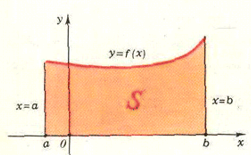
\includegraphics{img1.png}
    \label{fig:img1}
\end{figure}

Пример 1. \textit{Найти площадь фигуры, ограниченной линиями $y=1-x^2$ и $y=0$.}

Можно считать, что эта фигура ограничена осью абсцисс, прямыми $x=-1$, $x=1$ и графиков функции $y=1-x^2$ (рис. \ref{fig:img2}), поэтому по формуле~\eqref{eq:1} ее площадь 

\[S=\int_{-1}^1(1-x^2)dx.\]

\noindent Так как первообразной для функции $f(x)=1-x^2$ является функция 

\[F(x)=x-\frac{x^3}{3},\]

\noindent то

\[S=(x-\frac{x^3}{3})\Bigr\rvert_{-1}^1=\frac{4}{3}.\]

Вы видите, что в этом примере нам не пришлось прибегать ни к каким "ухищрениям": для решения задачи оказалось достаточным воспользоваться готовыми формулами. Но так бывает далеко не всегда.

\section{Аддитивность}
Решать более сложные задачи на вычисление площадей помогает свойство \textit{аддитивности} площадей. Оно "разрешает" разбить данную фигуру на части и подсчитать площадь всей фигуры как сумму площадей этих частей.

\begin{figure}[H]
    \centering
    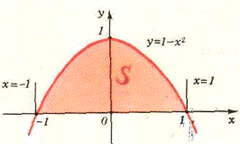
\includegraphics{img2.png}
    \label{fig:img2}
    
\end{figure}

\section{Раздел 2. Вероятность}
--Неважный ход, приятель, ... Вы, сударь, получите лошадей с полной сбруей. 

Торжествующий англичанин даже не потрудился смешать кости; его уверенность в победе была так велика, что он бросил их на стол не глядя. Д'Артаньян отвернулся, чтобы скрыть досаду.

--Вот так штука, - как всегда, спокойно проговорил Атос. --Какой необыкновенный ход! Я видел его всего четыре раза за всю мою жизнь: два очка!

Англичанин обернулся и онемел от изумления: Д'Артаньян обернулся и онемел от радости".

Давайте, и мы с вами бросим несколько раз пару костей -- кубиков из детских игр с цифрами или точками (очками) от 1 до 6 на гранях -- и посмотрим, часто ли выпадают две единицы. Чтобы различить эти кубики, один из них закрасим красной краской, а другой -- синей. В таблице \ref{tab:tab1} приведены результаты 36 бросаний красного и синего кубиков, выполненных нами. 

\begin{table}[H]
    \centering
    \begin{tabular}{|c||c|c|c|c|c|c|}
        \hline
        \diagbox[]{\textbf{кубики}}{\textbf{очки}}& 1 & 2 & 3 & 4 & 5 & 6 \\
        \hline
        \hline
        красный & 5 & 6 & 6 & 6 & 7 & 6 \\
        \hline
        синий   & 6 & 6 & 5 & 4 & 8 & 7 \\
        \hline
    \end{tabular}
    \caption{Появление отдельных очков при 36 бросаниях двух кубиков}
    \label{tab:tab1}
\end{table}

У Вас, конечно, получатся другие результаты, но если вы сведете свои результаты в таблицы (2 и 3), то скорее всего выводы будут те же, что и у нас.

\subsection{Выводы}
\begin{enumerate}
    \item Дубль 1--1 выпадает не часто (у нас -- один раз из 36);
    \item Разные очки выпадают примерно одинаково часто, в среднем -- в 1/6 части случаев каждое.
    \item Сумма очков на двух костях обычно заключена в пределах от 5 до 9.
    \item Если увеличить число бросаний, то отмеченные закономерности проступят еще более четко. Чем больше число бросаний, тем меньше будут...
\end{enumerate}

\end{multicols}
% \end{document}
